\subsection{Pulsars}

The first neutron star to be ever discovered by Jocelyn Bell in 1967 was in fact not just an ordinary neutron star, but was a pulsar. A pulsar is a neutron star star emits electromagnetic radiation from it's magnetic poles. Due to the rotation of the pulsars, the beams appear to be pulsating, similar to a lighthouse. Because their rapid pulse of radio emission is so predictable, a large array of well-understood pulsars can be used to measure extremely subtle abnormalities, such as gravitational waves. Pulsars are used as a timing clock to detect gravitational waves. Knowing the average time required for the pulsar signal to reach earth, the difference between when the pulsar signals should arrive, and when they do arrive, can signal a gravitational wave. A pulsar is depicted in \cref{fig:pulsar_image1}

\begin{figure}[h]
\centering
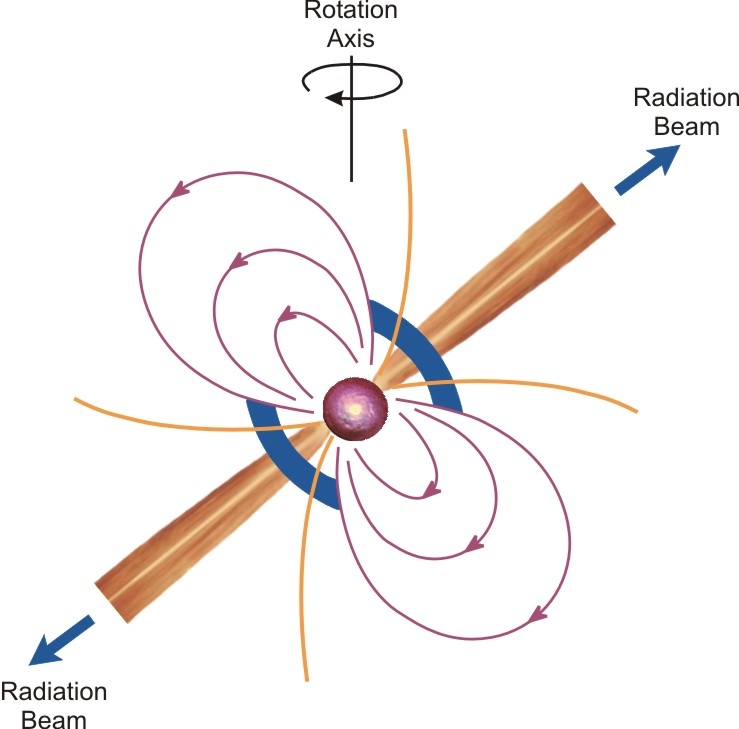
\includegraphics[height=0.5\textwidth, width=0.5\textwidth]{images/pulsar.jpg}
\caption{\small Artistic representation of a Pulsar; Credit: National Radio Astronomy Observatory}
\label{fig:pulsar_image1}
\end{figure}

Pulsars have high magnetic field and as a result, electrons and other subatomic particles are accelerated at very high speeds ($\approx$ the speed of light) causing them to emit beams of radio waves and other forms of radiation. As the pulsar rotates, the radiation beam rotates, and when the beam intersects with earth, we see it.

